\chapter{Kinematics}
	The study of \de{kinematics} of mechanisms are useful in order to define relative positions of bodies, reconstruct body position/orientation from sensor and optimise body position/orientation evolution over time.
	
	To describe \de{pose} and \de{attitude} (orientation) of a body in the space is better starting of with the notation of points; in particular any point $P$ in a dimensional space (for practical MBD application the 3D environment $\R^3$ is considered) can be described by a vector $\vett{v}$ that can be regarded as linear combination of the canonical base $\{\hat{\vett e_1},\hat{\vett e_2},\hat{\vett e_3}\}$:
	\begin{equation}
		\vett v := x \hat{\vett e_1} + y \hat{\vett e_2} + z \hat{\vett e_3}
	\end{equation}

	To describe a body, determining it's \textbf{configuration}, we can use a set of parameter such specific points of the body itself or some vectors on it.
	
	\paragraph{Rigid bodies} A \textbf{body} is defined as \de{rigid} if the distance between any it's two point and the angle of any two vector are constant in time (or the difference is so small that can be neglected) regardless of external forces exerted on it; mathematically a body is rigid if
	\begin{equation}
		\overrightarrow{P_1P_2} = \textrm{constant} \quad \textrm{ and } \quad \angle \{ \overrightarrow{P_1P_2},\overrightarrow{P_1P_3}\} = \textrm{constant} \hspace{2cm} \forall P_1, P_2, P_3 \textrm{ points} \in \textrm{body}
	\end{equation}

\section{Rotational matrix approach}
	The \de{rotational matrix} is an approach that's used to solve kinematic problems of multi-body mechanical systems.
	
	Considering a mono-dimensional case on where we want to describe a point lying on an axis, in order to define it's position is necessary to determine a \de{reference frame} on which we can define the position $x$ of the point respect to such origin; figure \ref{fig:kin:mono} shows that different reference frames can result in different coordinates of the point.
	
	\begin{SCfigure}[2][bht]
		\centering 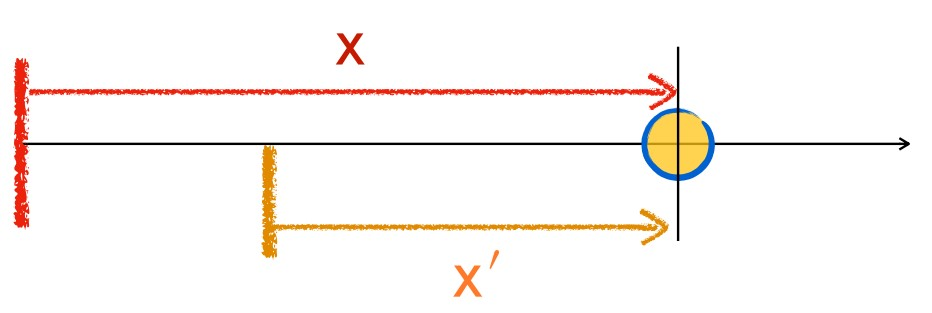
\includegraphics[width=6cm]{monodim}
		\caption{representation of the position of a point moving on one axis using two different reference frames (red and orange).} \label{fig:kin:mono}
	\end{SCfigure}
	
	Extending the case of a planar body, it's \textbf{configuration} $q$ can be described by defining a position (two \textit{spatial} coordinates $x,y$) and orientation ($\theta$) respect to a reference frame. Bodies are described using local reference frames where for example a point $\vett P_1^b$ is described. In order to define the position $\vett P_1$ in the global reference frame is so mandatory to know the configuration $\vett q = (x_0,y_0,\theta)$ of the body respect to the global coordinates (as shown in figure \ref{fig:kin:spatial}).
	\begin{SCfigure}[2][bht]
		\centering 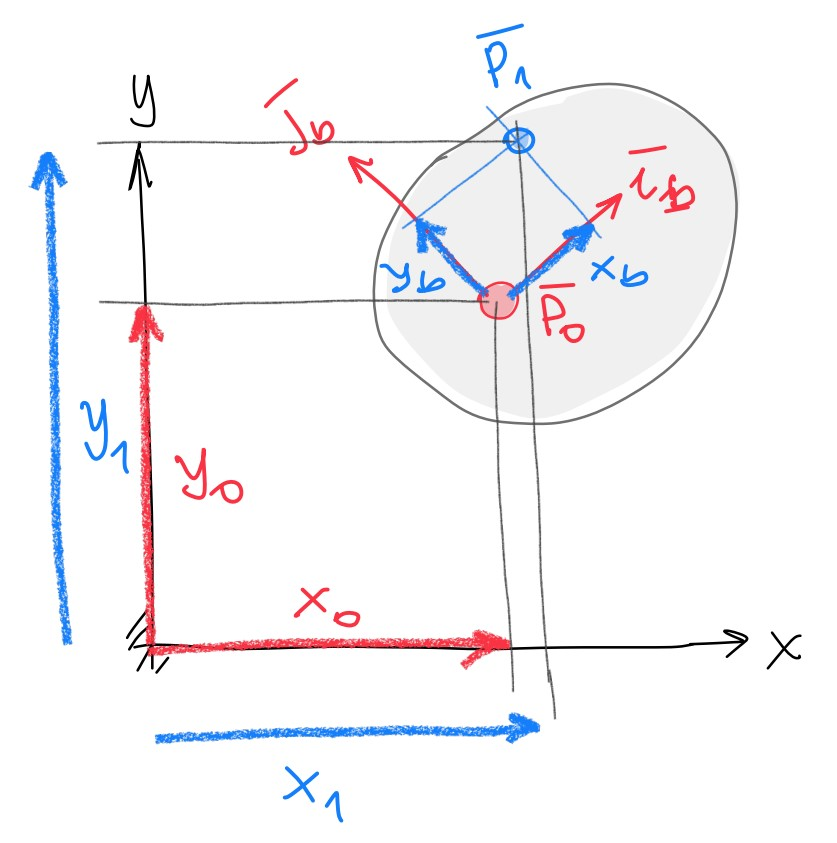
\includegraphics[width=5cm]{planarref}
		\caption{reference frames used for determining the position of a point/vector in the "global" frame knowing it's local coordinates.} 
		\label{fig:kin:spatial}
	\end{SCfigure}
	
	In this case we can see that the \textbf{point} can be described in the global reference frame as $\vett P_1 = (x_1,y_1)$ knowing it's local coordinates $\vett P_b (x_b,y_b)$ and it's configuration $\vett q = (\vett P_0,\theta)$ as
	\begin{equation} \label{eq:kin:2drototrans}
	\begin{split}
		\vector{x_1 \\ y_1} & = \vector{x_0 + x_b \cos \theta - y_b \sin\theta \\ y_0 + x_b\sin\theta + y_b\cos\theta} = \vector{x_0 \\ y_0} + \matrix{\cos\theta & \sin\theta \\ -\sin\theta\ & \cos\theta} \vector{x_b \\y_b} \\
		\vett P_1 & = \vett P_0 + \rot \vett P^b
	\end{split}
	\end{equation}
	
	If we now define $\overrightarrow{P_1 P_0} = \vers i_b $ the versor (a vector such that $\|\vers i_b\|=1$) aligned to the $x$ coordinate axis, we have that it description in the global reference system can be computed by determining $\vett P_1 - \vett P_0$ resulting in
	\[ \vers{i}_b = \vector{\cos\theta \\ \sin\theta} \]
	If we instead would have considered the versor $\vers j_b$ aligned to the $y$ axis what we would have obtained is the vector $(-\sin\theta ,\cos\theta)$. We can so now see that $\vers i_b$ and $\vers j_b$ are representing the columns of the \de{rotation matrix} $\rot$ firstly shown in equation \ref{eq:kin:2drototrans}. This matrix, in a more general case, contains the expression of the verso of the local frame measured in the global one and they generate a \de{base}, a set of vector $\{\vers e_1,\vers e_2, \vers e_3\}$ characterized by having:
	\[ \vers e_i\cdot \vers e_j = \begin{cases}
		1 & i = j \\ 0 & i \neq j 
	\end{cases} \hspace{1.5cm}  \textrm{and} \hspace{1.5cm} \vers e_1 \cdot \big(\vers e_2\times \vers e_3\big) = 1\]
	where the second condition represent the \textit{right-hand rule}. We so define \de{world/ground} \textbf{reference frame} as the fixed one on respect with \de{local/moving} reference frames are described (and usually are attached to bodies in the system). Given so the \textbf{rotational matrix} $\rot$ that describes the rotation of the local system respect to the world frame and the origin $\vett x_0$ of the local system (respect to ground) we have that the coordinates of point in the moving reference system $\vett x^b$ relates to the absolute space position $\vett x^w$ using equation
	\begin{equation} \label{eq:kin:directrototrans}
		\vett x^w = \vett x_0 + \rot \vett x^b
	\end{equation}
	Such equation can be inverted to determining
	\begin{equation} \label{eq:kin:inversrototrans}
		\vett x^b = \rot^{-1} (\vett x^w -\vett x_0) = \rot^{-1} \vett x^w - \rot^{-1} \vett x_0
	\end{equation}
	
	\paragraph{Inverse rotation} Rotational matrix $\rot$ belongs to the \de{special orthogonal matrix} $SO(N)$ space characterized by having
	\begin{equation}
		\det \rot = 1 \hspace{1.5cm} \textrm{and} \hspace{1.5cm} \rot^{-1} = \rot^t \quad \Rightarrow \quad \rot^{-1} \rot = \rot^t \rot= \I
	\end{equation}
	where so the inverse corresponds to the transposed of the matrix: this consideration is very useful because it allows to better perform inverse operations.
	
	\subsection{Transformation matrix}
		A good way to describe roto-translation as shown in equation \ref{eq:kin:directrototrans} and \ref{eq:kin:inversrototrans} is by using the \de{transformation matrix} $\rf{}$ notation, where all the calculation are condensed in the $4\times 4$ matrix described as
		\begin{equation}
		\begin{aligned}
			\ref{eq:kin:directrototrans} & \mapsto \vector{x_w \\ y_w \\ z_w \\ 1} = \matrix{ \begin{array}{c c c | c}
					&&& x_0 \\
					&\rot&& y_0 \\
					&&& z_0 \\ \hline
					0&0&0&1
			\end{array}} \vector{x_b \\ y_b \\ z_b \\ 1} \\
			\ref{eq:kin:inversrototrans} & \mapsto \vector{x_b \\ y_b \\ z_b \\ 1} = \matrix{ \begin{array}{c c c | c}
				&&& \\
				&\rot^{-1}&& -\rot^{-1} \vett O^w \\
				&&& \\ \hline
				0&0&0&1
		\end{array}} \vector{x_w \\ y_w \\ z_w\\ 1}
		\end{aligned}
		\end{equation}
		where $\vett O^w = (x_0,y_0,z_0)$ is the origin of the local reference frame respect to ground. With this definition the \textbf{reference frame} is the one characterized by having a transformation matrix of the form
		\[ \rf{}^w = \matrix{ \begin{array}{c c c | c}
				&&&0 \\
				&\I&& 0 \\
				&&& 0\\ \hline
				0&0&0&1
		\end{array}} \]
		
		\paragraph{Operation between points and vectors} While performing operation with points and/or vectors it necessary to understand if such operation is feasible (having a \textit{physical meaning}) or not; in particular we have that
		\begin{align*}
			\textrm{point} &- \textrm{point} \quad && \mapsto \quad \textrm{vector} \\
			\textrm{point} &+ \textrm{vector} \quad && \mapsto \quad \textrm{point} \\
			\textrm{vector} &\pm \textrm{vector} \quad && \mapsto \quad \textrm{vector} \\
			\textrm{point} &+ \textrm{point} \quad && \mapsto \quad \textrm{nothing} 
		\end{align*}
		
		\subsubsection{Order of transformation} 
		Local frames of multi-body systems are usually realised by performing multiple \textit{recursive} roto-traslation of reference systems. An important think to remember that the application of transformation matrix is a non-commutative operation, meaning that given the reference frame $\rfw$ and any two transformation matrix $\rf 1$ and $\rf 2$ we have that
		\[ \rf 1 \rf 2 \neq \rf 2 \rf 1 \]
		Observe that the product of any 2 (or more) reference frames $\rf i \rf j$ generates a new transformation matrix that allow to relates this new reference frames to the global coordinates.
		
		\paragraph{Pure translation} If we consider a reference frame $\rf 2$ defined as pure translation of a frame $\rf 1$ (that's also a pure translation of a world reference frame $\rfw$), as shown in figure \ref{fig:kin:translation}, defined by the transformation matrix 
		\[ \rf 1 = \transformationmatrix{ &&& x_{01}^w \\ & \I&& y_{01}^w \\ &&& z_{01}^w \\ \hline 0 & 0 & 0 & 1 } \hspace{2cm} \rf 2 = \transformationmatrix{ &&& x_{02}' \\ & \I&& y_{02}' \\ &&& z_{02}' \\ \hline 0 & 0 & 0 & 1 } \]
		in order to describe the second reference frame into global coordinate system we have to perform the operation $\rf 1 \rf 2$. Performing algebraically the operation we indeed retrieve the intuitive result of a transformation matrix $\rf 2^w$ with no rotation ($\rot = \I$) and center of the base in  $\vett x_1^w + \vett x_2'$, in fact
		\[ \rf 2^w = \rf 1\rf 2 = \transformationmatrix{ &&& x_{01}^2 + x_{02}' \\ & \I&& y_{01}^2 + y_{02}' \\ &&& z_{01}^2 + z_{02}' \\ \hline 0 & 0 & 0 & 1 } \]
		
		\begin{SCfigure}[2][bht]
			\centering 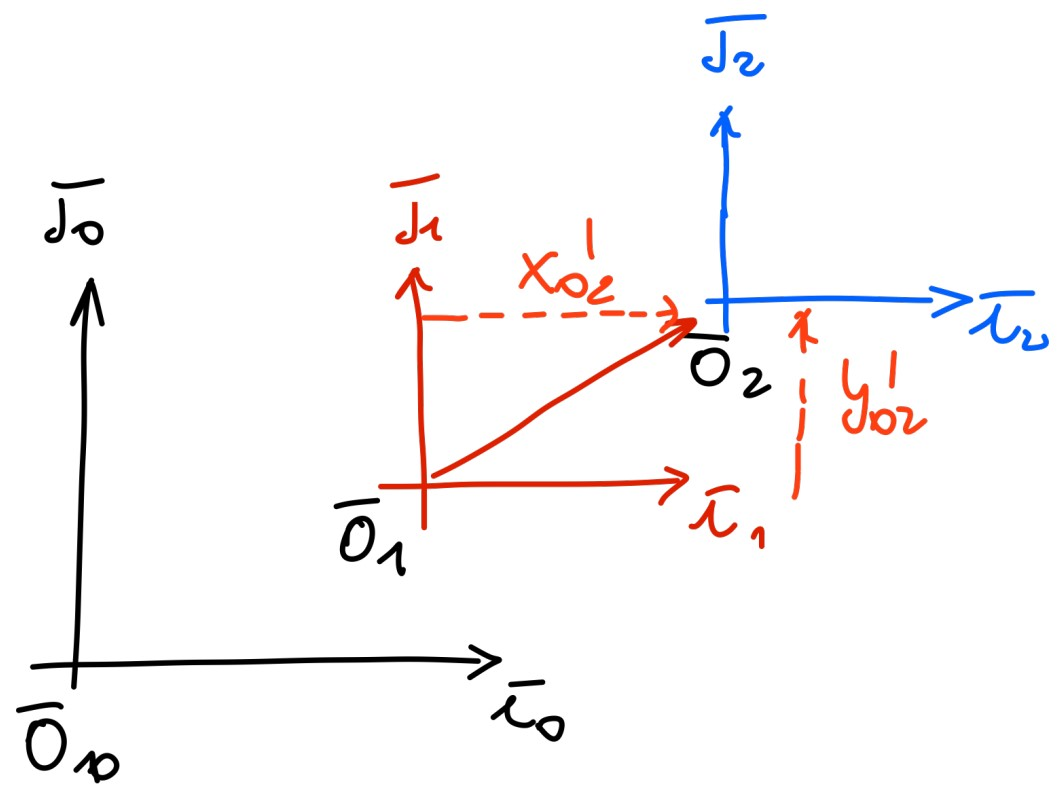
\includegraphics[width=5cm]{translationframe}
			\caption{multiple transformations of pure translation; in this case, for sake of simplicity, the planar case has been considered.} \label{fig:kin:translation}
		\end{SCfigure}
	
		\paragraph{Pure rotation} Considering a reference frame $\rf 2$ that a pure rotation (along the $z$ axis) of an angle $\beta$ respect to a reference frame $\rf 1$ characterized by a pure rotation of angle $\alpha$ respect to the reference frame $\rfw$ (figure \ref{fig:kin:rotational}), their transformation matrix are
		\[ \rf 1 = \transformationmatrix{\cos \alpha & -\sin \alpha & 0 & 0 \\ \sin\alpha & \cos \alpha & 0 & 0 \\ 0 & 0 & 1 & 0 \\ \hline 0 & 0 & 0 & 1} \hspace{2cm} \rf 2 = \transformationmatrix{\cos \beta & -\sin \beta & 0 & 0 \\ \sin\beta & \cos \beta & 0 & 0 \\ 0 & 0 & 1 & 0 \\ \hline 0 & 0 & 0 & 1} \]
		In order to determine the transformation of the second reference frame respect to the ground we so have to compute the product $\rf 1 \rf 2$ between the transformation matrix, hence
		\[ \rf 2^w = \rf 1 \rf 2 = \transformationmatrix{\cos \alpha \cos \beta -\sin\alpha\sin\beta & -\cos \alpha \sin \beta -\sin\alpha \cos \beta & 0 & 0 \\ \sin\alpha\cos\beta + \cos\alpha\sin\beta & -\sin\alpha\sin\beta + \cos\alpha\cos\beta & 0 & 0 \\ 0 & 0 & 1 & 0 \\ \hline 0 & 0 & 0 & 1} \]
		Using so Prostaferesi's equation involving the sum of the argument in (co)sine functions we obtain the intuitive result of a pure revolution of $\alpha + \beta$ along the $z$ axis:
		\[ \rf 2^w = \transformationmatrix{\cos (\alpha +\beta) & -\sin (\alpha + \beta) & 0 & 0 \\ \sin(\alpha + \beta) & \cos (\alpha + \beta) & 0 & 0 \\ 0 & 0 & 1 & 0 \\ \hline 0 & 0 & 0 & 1} \]
		\begin{SCfigure}[2][bht]
			\centering 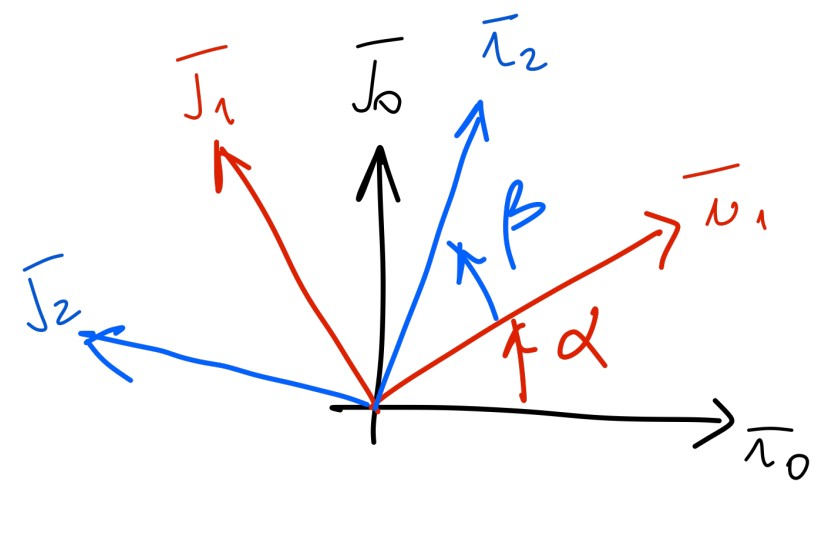
\includegraphics[width=5cm]{rotational}
			\caption{multiple transformations of pure rotation revolving the $z$ axis.} \label{fig:kin:rotational}
		\end{SCfigure}
		
		\paragraph{Rotation and translation} In the case of pure rotation/translation the reference frame that we have obtained was the same if we would have applied the transformation in reversed order, however this are only particular case. If we consider a translation $\rf 1$ and a rotation $\rf 2$ defined by matrix
		\[  \rf 1 = \transformationmatrix{ &&& x_{01}^w \\ & \I&& y_{01}^w \\ &&& 0 \\ \hline 0 & 0 & 0 & 1 }  \hspace{2cm} \rf 2 = \transformationmatrix{\cos \alpha & -\sin \alpha & 0 & 0 \\ \sin\alpha & \cos \alpha & 0 & 0 \\ 0 & 0 & 1 & 0 \\ \hline 0 & 0 & 0 & 1} \]
		Intuitively the reference frame obtain by firstly applying the translation ($\rf 1$) is different from the one obtained by rotating first ($\rf 2$), in fact by performing the matrix calculations we obtain
		\[ \rf 1 \rf 2 = \transformationmatrix{ &&& x_{01}^w \\ &\rot_\alpha && y_{01}^w \\ &&& 0 \\ \hline 0&0&0& 1} \hspace{1.5cm} \rf 2 \rf 1  = \transformationmatrix{ &&& x_{01}^w \cos\alpha  - y_{01}^2 \sin\alpha \\ &\rot_\alpha && x_{01}^2 \sin\alpha + y_{01}^w \cos\alpha \\ &&& 0 \\ \hline 0&0&0& 1}  \]
		
		
		\begin{figure}[bht]
			\centering 
			\begin{subfigure}{0.48\linewidth}
				\centering 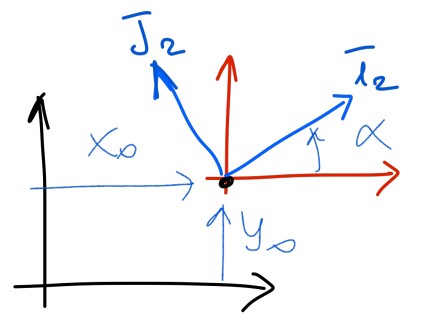
\includegraphics[width=5cm]{rototrans-1} \caption{}
			\end{subfigure}
			\begin{subfigure}{0.48\linewidth}
				\centering 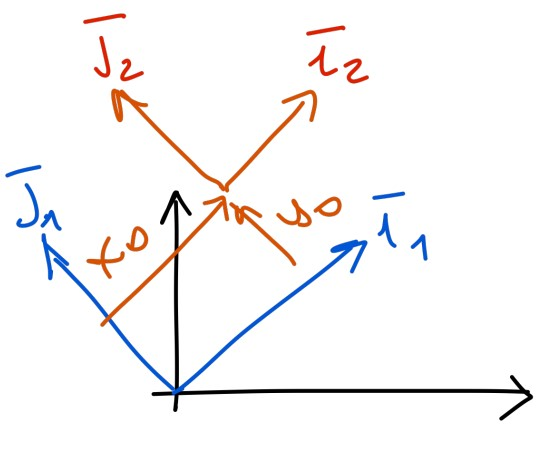
\includegraphics[width=5cm]{rototrans-2} \caption{}
			\end{subfigure}
			\caption{reference frame obtained by first translating and than rotating $(a)$ and first rotating and then translating $(b)$.} \label{fig:kin:transforder}
		\end{figure}
	
	
	
	
	
	
	
	
	
	
	